\section{Implementation}

\subsection{String alignment}
The data containing the roles and the string describing the actual role contains superfluous information, e.g. the id of the actor, the id of the movie . The string describing the role can for instance contain information defining what specific policeman it was. In order to generalise the roles such information is removed, e.g. there is no difference between policeman \#1 and policeman \#2 in the cleaned dataset. Additionally unspecified roles are deleted. As an example multiple people has had a role playing themselves. Such a role is defined as “Themselves” in the dataset, which is very general and not the actual role, hence these are deleted. Other similar roles, e.g. himself, herself, extra or additional are removed as well. Some roles define which year the role was from. This information is also removed. Finally, many of the string describing the roles are empty. The entries are deleted.

\subsection{Data processing}
There are multiple ways to handle the data that needs to be processed.
One approach is to load all the data into the RAM. This technique is very demanding on the RAM, since everything is stored. Storing everything in the RAM has some clear advantages e.g. being able to go back and forth in the data or reading the same subset of the data multiple times. However if the size of the data exceeds the amount of RAM available, one might experience severe performance implications, due to e.g. memory swapping.
Some datasets have a size which makes it impractical, sometimes even impossible, to store them in the RAM. This constraint leads to another approach, which is to stream the data. Streaming the data has advantages as well as disadvantages. Only a fraction of the whole data is stored in the RAM, imposing no extraordinary demand to the size of the available RAM. Only storing part of the data makes it cumbersome, and to some extent impossible, to go back and forth in the data.

\subsection{Practical space consumption}
The following logarithmic graph is the number of map entries used by Misra Gries, reservoir sampling and the naive solution based on the concrete data set. The vertical axis is space consumption and the horizontal axis is \(\alpha\). Only the naïve solution is dependent on the size of the concrete example and not on \(\alpha\). The reservoir sampling algorithm is linear dependent on the threshold.
\begin{figure}[H]
	\centering
	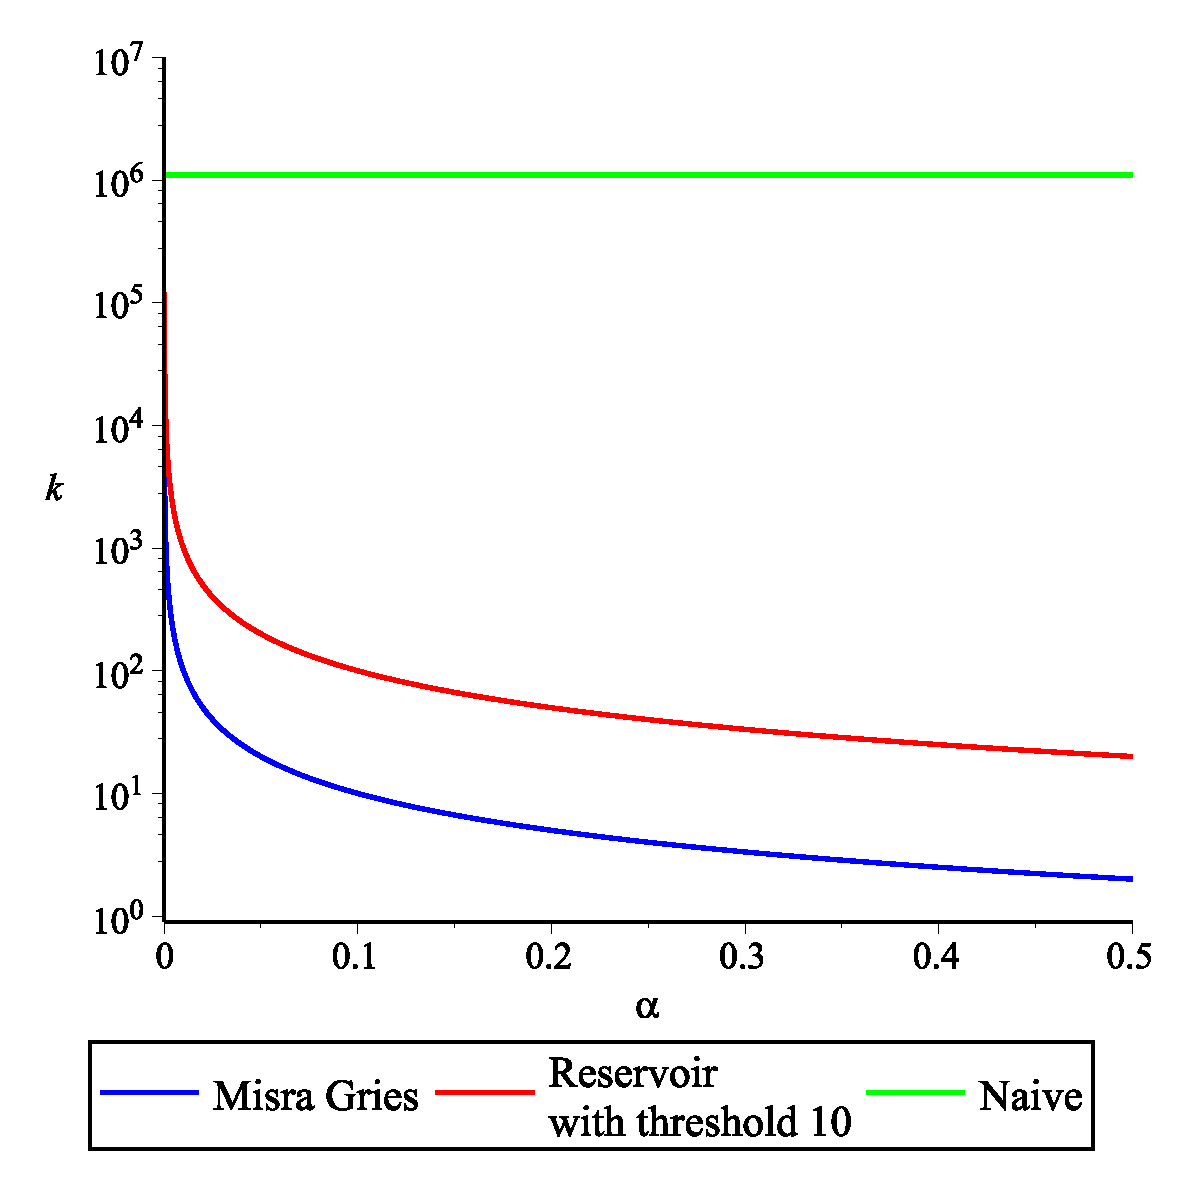
\includegraphics[width=350px]{img/streamingMemoryGraph.eps}
	\caption{Space consumption}
	\label{fig:space_consumption}
\end{figure}
As seen in figure~\ref{fig:space_consumption} the space used by the naïve solution is 1000 times as large as the space used by Misra Gries and reservoir sampling. when looking for elements in Hwith =0.001. The size of the data stream is approximately 2.3 million.
